\documentclass[iop,apj]{emulateapj}
\usepackage{amsmath,amssymb,amstext}

\usepackage[breaklinks,colorlinks,citecolor=blue,linkcolor=magenta]{hyperref} 
\renewcommand*{\sectionautorefname}{Section}
\usepackage[all]{hypcap} %Links go to figures; breaks on deluxetables (use \capstartfalse \capstarttrue to fix it)

\usepackage{aas_macros}
\usepackage{natbib}
\bibliographystyle{apj}

\shorttitle{Short Title}
\shortauthors{Author et al.}

\begin{document}

\title{Detecting Active Asteroids/Comets from OSSOS survey images}
\author{Authors}
\affil{Affiliations}

\begin{abstract}
Abstract.
\end{abstract}

\keywords{keywords}
\maketitle

\section{Introduction}
% so far, im not making a point of using good wording
% definietly have to go back and add in citations

The active asteroids are small bodies in the main asteroid belt which have transient dust emission producing comet-like comae and tails. Unlike comets, which originate in the Kuiper Belt and Oort cloud and have been scattered inwards by gravitational effects, the active asteroids have  stable orbits confined to the main belt and likely formed in the same location as they reside presently \citep{sheppard14}. For objects which formed in the the outer region of the main belt, beyond the snow line, the crystallized water ice which was present at the time of formation and not exposed to primordial heating may still remain in reservoirs beneath the surface \citep{sonnett11}.  According to models done by \citet*{fanale89},  beyond heliocentric distances of 2.4 AU ice can be protected against sublimation by a "relatively thin" surface regolith  of depth 1 -- 100 m for the entire age of the solar system. If the ice layer were to be exposed to sub solar heating,  sublimation could be triggered,  ejecting dust particles from the surface producing a coma.  %Objects in the main asteroid belt which are driven by sublimation are also named Main Belt Comets (MBCs). 
The source of the dust emission may be different for each object and could include ice sublimation, impact ejecta, rotational instabilities due to YORP torques, or a combination of several effects. \citep{hsieh15}. %; these objects are known as disrupted asteroids. 
As the source of the observed activity may not be a result of cometary ice sublimation, these objects are better known as active asteroids. Main belt comets are a subset of this group where ice sublimation is thought to be the source of the dust emission. 

% As the presence of ice in the inner solar system could be important for determining the chemistry of the early solar nebula and planet formation, it is worth while to determine what the source of the activity is. 
% impacts inferred from observed large brightening and quick fading 
% sublimation inferred from prolonged or periodic activity during perihelion passage, Hsieh et al 2010, 2011

%The ejected dust would form a coma around the object, and radiation pressure affects would then (preferentially) push the smaller particles away from the asteroid forming a tail.

%Sublimation driven active asteroids differ from comets in that the comets, having larger ice reservoirs, would have stronger sublimation events which could eject larger debris. The cometary tail would then be longer lived as the larger debris would be less effected by the radiation pressure, and thus dissipate slowly. It is also possible, however, that prolonged activity is a result of ongoing ejection of small, fast dissipating particles. \cite{TEST} 

Since the first discovery of an active main-belt asteroid, 133P/Elst-Pizarro, several attempts have been made to identify new objects of this type; at present, eighteen objects have been identified \citep{jewitt15}. A comprehensive review of such searches can be found in \citep{hsieh15}.  A persistent challenge to this effort is that the detection of the coma or tails is highly dependent on the magnitude constraints of the survey for small dark objects. As most asteroids fall near the limiting magnitudes of the survey in which they are discovered \cite{jewitt15}%(is this cite necessary?)
, objects which are larger, closer, or have higher albedo are preferentially detected and any dust emission would be more easily apparent. The active fraction of identified active asteroids greater than 1 km to main belt asteroids greater than 1 km is $f \, \sim \, 10^5$, and describes a strong lower limit as many objects are yet undetected. \citep{jewitt15} %From a study of 30,000 objects observed near perihelion, \cite{} Hsieh et all (2015) concluded that $f \, \sim \, 10^4$ for asteroids which are active at any instant in the outer belt.

The data set provided by the Outer Solar System Origins Survey (OSSOS) is valuable for detecting activity in main belt objects due to its low limiting magnitude of 24.5 mag as well as wide field coverage of both the ecliptic plane and low inclinations. Observations of the known objects in this survey could allow for serendipitous discoveries of active dust emission which was previously to faint to detect. 



% WHAT IS NEW, BETTER, DIFFERENT ABOUT OSSOS???


\section{Observations}

Observations taken by OSSOS with the Canada-France-Hawaii telescope (CFHT) MegaPrime wide-field optical imaging facility have been collected since 2013 at the summit of Mauna Kea, Hawaii. The wide-field imager, MegaCam, consists of a 36 CCD image plane, each 2048 x 4125 CCD with resolution of 0.185"/pix. This covers a field of  roughly 1$^{\circ}$ x 1$^{\circ}$ on the sky. Each block of data taken by OSSOS consists of a mosaic of 21 segments of one-square-degree sky coverage, and at present covers two orbital phase spaces on the plane of the ecliptic, and two off plane at low inclinations. MegaCam observes in the optical to near infrared with filters u*, g', r', i', and z'. Of these, r' and u* are the best suited filters for observing main belt objects, and the analysis presented only includes observations made using these filters (reword!). 

% how is the image data calibrated? filters, S/N? MOPS?



As the identified active asteroids do not share a specific phase space (refer to Figure 1) the analysis was not constrained to just the main belt or plane of the ecliptic, but for all known objects with heliocentric distances beyond the inner belt ( a > 2.064 AU), inclinations below 40$^{\circ}$, and eccentricity less than 0.45. 
For all of the known asteroids in the main belt with semimajor axis beyond the inner belt
% to detect objects in the main asteroid belt, objects with semimajor axis 2.064 < a < 3.277 AU, e < 0.45, i < 40 deg
% PSF detections
% cuts, identifying process





\acknowledgments{
  Acknowledgments. 
}

\bibliographystyle{plainnat}
\bibliography{mbc_paper}

\begin{figure}[!htb]
\minipage{0.5\textwidth}
    \centering
    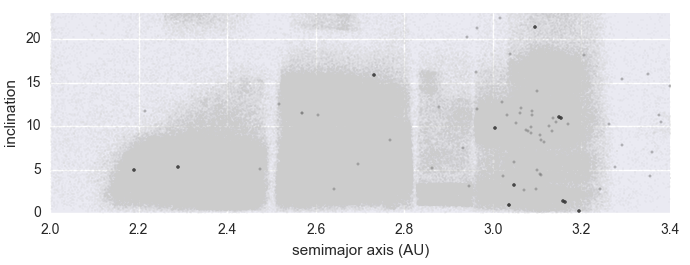
\includegraphics[height=4cm]{inc_a.png}
    \caption{Inclination of objects as a function of semimajor axis. }\label{fig:1}
\endminipage
\minipage{0.5\textwidth}
    \centering
    \includegraphics[height=4cm]{InnerDetector.png}
    \caption{The ATLAS Pixel System}\label{fig:2}
\endminipage\hfill
\end{figure}

\end{document}



